\documentclass[a4paper,11pt]{article}

\usepackage{lmodern}
\usepackage[T1]{fontenc}
\usepackage[polish]{babel}
\usepackage{graphicx}
\graphicspath{ {./images/} }

\begin{document}

\selectlanguage{polish} % Explicitly select Polish language

\begin{figure}[h]
\centering

\includegraphics{logo_politechniki_lubelskiej.jpg}
\end{figure}

\begin{center}
\textbf{\large Wydział informatyki i elektrotechniki}

Zarządzanie bazami SQL i NoSQL

Michał Gagoś

Rok 3 studia niestacjonarne

Grupa 6.3

Zajęcia odbywają się w soboty o 10:30
\end{center}


\pagebreak
\part{Baza SQL}
\section*{Opis Problemu}
Serwis internetowy łączy sprzedawców aut z kupującymi. Pozwala on kupującym wyszukać porządane auto na bazie dużej ilości parametrów.
Ogłoszenia zawierają takie informacje jak cena, lokalizacja, moc, napęd, stan, przebieg i wiele innych.


\section*{Oprogramowanie}
W celu przechowywania i organizacji danych wykorzystamy bazę danych \textbf{PostgreSQL}.
Natomiast w celu poprawienia komfortu pracy podczas tworzenia projektu skorzystamy z systemu konteneryzacji \textbf{Docker}.
Pozwoli to na uniknięcie instalacji bazy danych \textbf{PostgreSQL} na systemie docelowym i zapewni świeże i przewidywalne środowisko za każdym uruchomieniem.

\pagebreak
\section*{Struktura Bazy Danych}
Infrastruktura bazy składa się z wielu tabel zapewniających spójne przedstawienie danych.
Ta sekcja ma na celu scharakteryzowanie użytych tabel.

\begin{itemize}
    \item \textbf{users} --- Tabela użytkowników serwisu.  Zawiera dane logowania, hasło w postaci hasha md5 i klucze obce prowadzące do profilu publicznego użytkownika i jego statystyk.
    \item \textbf{user\_details} --- Tabela profili publicznych użytkowników. Zawiera informacje takie jak opis profilu i link do zdjęcia profilowego.
    \item \textbf{user\_stats} --- Tabela statystyk użytkowników. Zawiera informacje do statystyk odnośnie ilości sprzedanych i kupionych przez użytkownika aut.
    \item \textbf{manufacturers} --- Tabela producentów samochodów. Zawiera nazwy producentów samochodów.
    \item \textbf{vehicles} --- Tabela modeli samochodów. Zawiera modele samochodów i ich informacje techniczne. Są to informacje zapewniane przez administratora serwisu w celu uniknięcia błędów ze strony użytkownika.
    \item \textbf{offers} --- Tabela ofert zamieszczonych w serwisie. Zawiera informacje o sprzedawanym samochodzie jak i klucze obce sprzedawcy i modelu samochodu.
    \item \textbf{user\_likes} --- Tabela łącząca użytkowników z polubionymi przez nich ofertami.
\end{itemize}

\section*{Diagram EER}
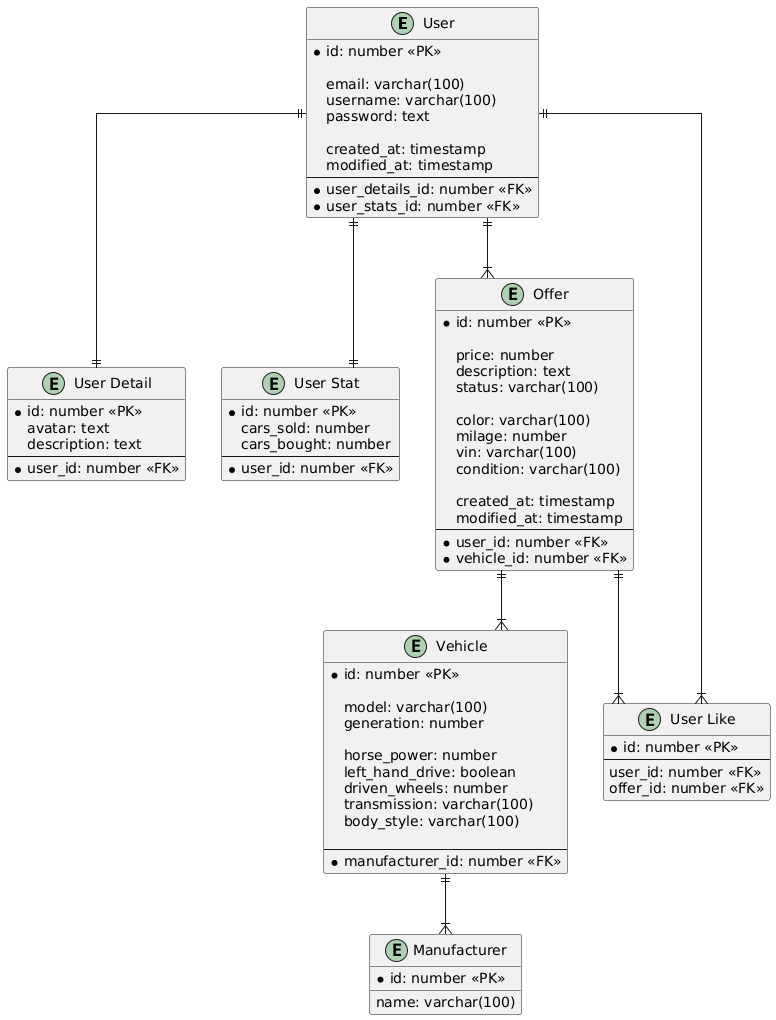
\includegraphics[width=\textwidth]{database.png}
\pagebreak

\section*{Wstawianie Danych}
W przypadku tego projektu dane są wstawiane z plików \textbf{.csv} z przykładowymi danymi wygenerowanymi przez sztuczną inteligencję.
\linebreak

Wstawianie danych z pliku \textbf{.csv} w bazie \textbf{PostgreSQL} odbywa się w następujący sposób:

\begin{verbatim}
COPY manufacturers(id,cars_sold,cars_bought)
FROM '/docker-entrypoint-initdb.d/data/user_stats.csv'
DELIMITER ','
CSV HEADER;
SELECT setval('user_stats_id_seq', (SELECT MAX(id) FROM user_stats));
\end{verbatim}

Możliwe też jest wstawianie danych ręcznie za pomocą języka \textbf{SQL}:

\begin{verbatim}
INSERT INTO manufacturers(name) VALUES ('Volvo');
\end{verbatim}

\section*{Przykłady Kwerend}
\subsection*{DDL --- Data Definition Language}
\begin{verbatim}
    CREATE TABLE user_likes (
        id SERIAL PRIMARY KEY,
        user_id INT NOT NULL,
        offer_id INT NOT NULL,
        
        CONSTRAINT fk_users FOREIGN KEY(user_id) REFERENCES users(id),
        CONSTRAINT fk_offers FOREIGN KEY(offer_id) REFERENCES offers(id)
    );

    DROP TABLE user_likes;
\end{verbatim}

\subsection*{DML --- Data Query Language}
\begin{verbatim}
    
\end{verbatim}

\subsection*{DCL --- Data Control Language}

\subsection*{TCL --- Transaction Control Language}

\pagebreak
\part{Baza NoSQL}

\end{document}
